\documentclass[12pt]{article}

%------------------------------------------------
% PAQUETES
%------------------------------------------------
\usepackage[utf8]{inputenc}
\usepackage[T1]{fontenc}
\usepackage[spanish]{babel}

\usepackage{amsmath,amssymb}
\usepackage{graphicx}
\usepackage{enumitem}
\usepackage{geometry}

\geometry{margin=2.5cm}

%------------------------------------------------

\begin{document}

\section*{Problema 2 - Versión 1}
Considere una circunferencia de radio $20,\mathrm{cm}$, en la cual se encuentra un sistema de dos cargas eléctricas, como se muestra en la figura. Las cargas tienen valores $q_1=12,\mu\mathrm{C}$ y $q_2=-6,\mu\mathrm{C}$.

\begin{enumerate}[label=\alph*)]
\item Dibuje y represente claramente el vector campo eléctrico producido por cada una de las cargas en los puntos $P_1$ y $P_2$, identificando cada vector según la carga que lo genera.

\item Determine el campo eléctrico neto generado por el sistema de cargas en el punto $P_1$, ubicado en el origen del sistema de coordenadas.

\item Determine el campo eléctrico neto generado por el sistema de cargas en el punto $P_2$, ubicado $30\,\mathrm{cm}$ sobre el centro de la circunferencia.


\end{enumerate}


\begin{center}
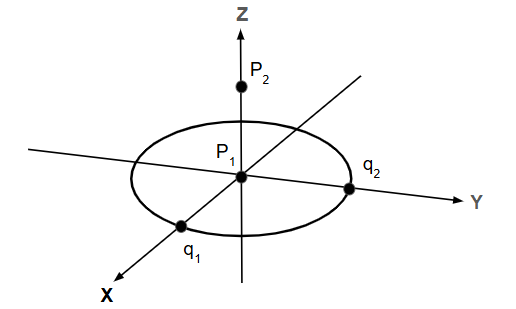
\includegraphics[width=0.65\textwidth]{imagen cargas.png}
\end{center}






\end{document}